% ============================================================
% Capitolo 6 — Timer TON (20260316 Timer TON.pdf)
% ============================================================
\chapter{Timer TON}
\label{cap:timer-ton}

\section{Definizione}
\begin{defn}[TON — Timer On Delay]
Function Block che implementa un ritardo all'accensione (\emph{turn-on delay}). La firma è \texttt{TON(IN, PT, Q, ET)}:
\begin{itemize}
    \item \textbf{Input}:
    \begin{itemize}
        \item \texttt{IN} (tipo \texttt{BOOL}): il segnale di «start»; quando viene posto a \texttt{TRUE} il timer inizia a contare;
        \item \texttt{PT} (tipo \texttt{TIME}): il «Prescribed Time», il tempo prescritto prima che venga emesso il segnale di timeout;
    \end{itemize}
    \item \textbf{Output}:
    \begin{itemize}
        \item \texttt{Q} (tipo \texttt{BOOL}): il segnale di timeout;
        \item \texttt{ET} (tipo \texttt{TIME}, «Elapsed time»): il tempo trascorso da quando il timer è partito.
    \end{itemize}
\end{itemize}
\end{defn}

\section{Comportamento nel tempo}
\begin{itemize}
    \item \textbf{Inizialmente}: \texttt{IN} = FALSE, \texttt{Q} = FALSE, \texttt{ET} = 0;
    \item \textbf{Appena \texttt{IN} diventa TRUE}: il tempo inizia a essere contato in millisecondi in \texttt{ET}, finché il suo valore non raggiunge \texttt{PT}; poi \texttt{ET} resta costante;
    \item \textbf{\texttt{Q} diventa TRUE} quando \texttt{IN} è TRUE \emph{e} \texttt{ET} è uguale a \texttt{PT}.
\end{itemize}

Casi di disattivazione:
\begin{itemize}
    \item se \texttt{IN} viene posto a FALSE \textbf{dopo} la scadenza di \texttt{PT}: \texttt{Q} torna FALSE e \texttt{ET} viene azzerato;
    \item se \texttt{IN} viene posto a FALSE \textbf{prima} della scadenza di \texttt{PT}: \texttt{Q} resta FALSE (non è mai scattato) e \texttt{ET} viene azzerato (il conteggio riparte da capo al prossimo fronte di \texttt{IN}).
\end{itemize}

\begin{figure}[htbp]
\centering
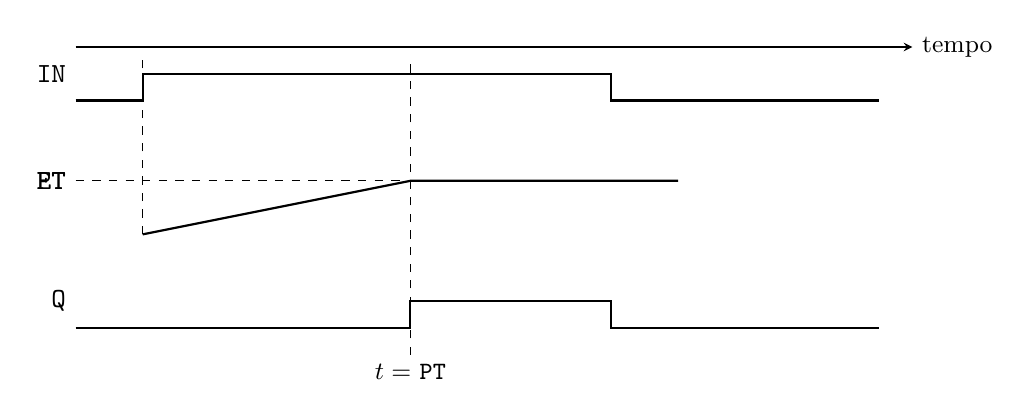
\begin{tikzpicture}[>=stealth, scale=0.85]
    % assi
    \draw[->] (0,4.6) -- (12.5,4.6) node[right] {\small tempo};
    % IN
    \node[anchor=east] at (0,4.2) {\texttt{IN}};
    \draw[thick] (0,3.8) -- (1,3.8) -- (1,4.2) -- (8,4.2) -- (8,3.8) -- (12,3.8);
    % ET
    \node[anchor=east] at (0,2.6) {\texttt{ET}};
    \draw[thick] (1,1.8) -- (5,2.6) -- (9,2.6);
    \draw[dashed] (5,0) -- (5,4.4);
    \draw[dashed] (1,1.8) -- (1,4.4);
    % PT line
    \draw[dashed] (0,2.6) -- (9,2.6);
    \node[anchor=east] at (0,2.6) {\texttt{PT}};
    \node[below] at (5,0) {\small $t = $ \texttt{PT}};
    % Q
    \node[anchor=east] at (0,0.8) {\texttt{Q}};
    \draw[thick] (0,0.4) -- (5,0.4) -- (5,0.8) -- (8,0.8) -- (8,0.4) -- (12,0.4);
\end{tikzpicture}
\caption{Timing diagram del TON: \texttt{ET} cresce linearmente finché raggiunge \texttt{PT}, allora \texttt{Q} sale; quando \texttt{IN} torna FALSE, \texttt{Q} scende e \texttt{ET} si azzera.}
\label{fig:ton-timing}
\end{figure}

\section{Programma semplice con timer TON}
Esempio d'uso tipico (con blocchi numerati come nelle slide):
\begin{itemize}
    \item il \textbf{blocco (1\ldots3)} viene eseguito finché \texttt{PT} non è trascorso e \texttt{Q} resta FALSE; poi \texttt{Q} diventa TRUE;
    \item il \textbf{blocco (4\ldots7)} viene eseguito \textbf{una sola volta}\ldots
    \item \ldots\ poiché porre \texttt{IN} a FALSE forza \texttt{Q} a FALSE (autodisattivazione: il ramo che scatta con \texttt{Q} = TRUE spegne il timer).
\end{itemize}

\begin{intuition}[Pattern d'uso]
Il pattern fondamentale è: \emph{chiamare} il timer ad ogni ciclo con \texttt{timer(IN := ..., PT := ...)}, \emph{testare} il timeout con \texttt{IF timer.Q THEN ...}, e \emph{resettare} il timer con \texttt{timer(IN := FALSE)} all'interno del ramo di timeout. Questo pattern è la base per gli \textbf{stati temporizzati} (Capitolo~\ref{cap:stati-temporizzati}).
\end{intuition}
